\documentclass{article}
\usepackage[utf8]{inputenc}
\usepackage[spanish, es-tabla]{babel}

%\graphicspath{ {/home/Juanpmd/Desktop/Images} }
%\hyphenation{op-tical net-works semi-conduc-tor}
\setlength{\parindent}{0em}
\setlength{\parskip}{1em}
\usepackage{cite}
\usepackage{url}
\usepackage{color}
\usepackage{graphicx}
\title{Proyecto Multimedia}
\author{Sebastian Lozano Herrera\\ sebaslh12@gmail.com \and Felipe Rojas Hernández\\ feliperojas12@hotmail.com}
\date{\ } 
\begin{document}
\maketitle
\section{Descripción}
El proyecto a desarrollar consiste en implementar un metodo de compresión y
descompresión de imágenes, utilizando para esto la transformada discreta del coseno y su inversa.
\section{Objetivo}
El objetivo es lograr la misma o mejor capacidad de compresión que se obtiene con el formato jpeg.
\section{Tecnologías}
\subsection{Back-End}
Para el desarollo del proyecto hemos escogido Python como el lenguaje de programación adicionalmente utilizaremos la librería Numpy para la manipulación númerica de las imágenes y Tkinter.
\newpage
\subsection{Front-End}
\begin{figure}[h]
\centering
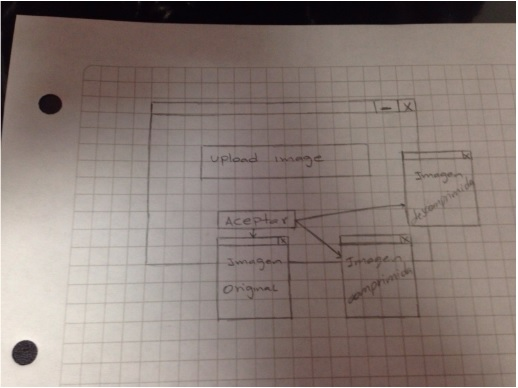
\includegraphics[width=\textwidth]{mockup}
\caption{Mockup primera versión}
\end{figure}

\end{document}